\documentclass{article}

\PassOptionsToPackage{numbers,compress}{natbib}
\usepackage[final]{neurips_2024}
\makeatletter
\renewcommand{\@noticestring}{}
\makeatother

\usepackage[T1]{fontenc}
\usepackage{amsmath}
\usepackage{amssymb}
\usepackage{booktabs}
\usepackage{graphicx}
\usepackage{microtype}
\usepackage{xcolor}
\usepackage{hyperref}
\usepackage[capitalize,noabbrev]{cleveref}
\usepackage{enumitem}
\usepackage{float}
\usepackage{subcaption}
\usepackage{wrapfig}
\usepackage{needspace}

\definecolor{reportblue}{HTML}{2563EB}
\definecolor{reportred}{HTML}{DC2626}
\definecolor{darkblue}{rgb}{0.10,0.20,0.55}
\hypersetup{
  colorlinks=true,
  citecolor=darkblue,
  linkcolor=darkblue,
  urlcolor=darkblue
}

\setlist[itemize]{leftmargin=*,topsep=2pt,itemsep=1pt,parsep=0pt}
\setlength{\emergencystretch}{1.5em}
\clubpenalty=10000
\widowpenalty=10000
\displaywidowpenalty=10000

\newcommand{\ppl}{\operatorname{PPL}}

\title{NanoCloud01: Data-Aware Continuation Training\\
for a 99M-Parameter Language Model}

\author{
  Yirui Miao \quad Fengfei Yu \quad Tianyue Zhang \quad Zavier Zhao\\
  University of California San Diego\\
  \texttt{y5miao@ucsd.edu, fey006@ucsd.edu, tiz052@ucsd.edu, zhz214@ucsd.edu}\\
  \url{https://github.com/ty1erz/cse251b-nanogpt}
}

\begin{document}
\maketitle
\raggedbottom
\setlength{\parfillskip}{0pt plus 0.3\linewidth}

\begin{abstract}
We study autoregressive language modeling under a strict 100M-parameter
submission limit. Starting from a nanoGPT-style baseline, we investigate three
coupled design axes: capacity allocation in compact Transformers, mixed-domain
training data, and optimization after the main pretraining schedule. Our model
family combines RoPE, RMSNorm, SwiGLU, tied embeddings, and optional
grouped-query attention (GQA). The final Model~2 has 99.03M parameters, 16
layers, and a 1:2 GQA ratio. It is trained on a 50/20/15/15 mixture of
FineWeb-Edu, Wikipedia, science, and books using a Muon--AdamW optimizer split.
Its first training stage reaches 21.163 public-validation perplexity after 38k
updates. Low-learning-rate continuation and dense checkpoint evaluation reduce
this to \textbf{18.768} at step 69.7k, which we select for the final
submission. Controlled comparisons show that data composition, optimizer
choice, and checkpoint selection are as consequential as architecture at this
scale.
\end{abstract}

\section{Introduction}
\label{sec:introduction}

\paragraph{Problem definition.}
The competition asks for a causal language model that predicts each GPT-2 BPE
token from its preceding context. The submitted model must contain at most
100M parameters, return logits over exactly 50,257 vocabulary entries, and
finish evaluation within the course time limit. Performance is measured by
token-level perplexity on a public validation set during development and a
hidden test set for the final ranking.

\paragraph{Problem significance.}
Compact language models are useful when memory, latency, privacy, or deployment
cost rules out a large hosted model. The same next-token objective supports
document completion, educational tools, coding assistance, retrieval
reranking, and on-device generation. The constrained setting is also
scientifically useful: because model size is fixed, improvements must come from
better capacity allocation, data, optimization, and engineering rather than
parameter scaling alone.

\paragraph{Technical challenges.}
The parameter cap creates direct competition among vocabulary embeddings,
depth, attention projections, and feed-forward width. Data presents a second
challenge: a single source may train efficiently yet generalize poorly to the
multi-domain evaluator. Long runs must also resume exactly, preserve optimizer
and loader state, and export an inference-compatible model. Finally, validation
performance near convergence is non-monotonic, so the last checkpoint is not
necessarily the best checkpoint.

\paragraph{Contributions.}
Our work makes four concrete contributions:
\begin{itemize}
  \item We compare three sub-100M decoder architectures that trade independent
  key/value capacity and residual width for depth.
  \item We implement a deterministic four-source loader and show that balanced
  multi-domain training outperforms single-source and overly FineWeb-heavy
  alternatives.
  \item We use Muon for hidden matrices and AdamW for embeddings and remaining
  parameters, improving early validation PPL by 8.6\% over AdamW alone.
  \item We reduce Model~2 PPL from 21.163 to 18.768 without changing its
  architecture, data mixture, or objective, demonstrating the value of
  low-rate continuation and checkpoint selection.
\end{itemize}

\section{Related Work}
\label{sec:related}

\paragraph{Compact Transformer design.}
Our models follow the decoder-only Transformer family
\citep{vaswani2017attention} and the minimal training interface popularized by
nanoGPT \citep{karpathy2022nanogpt}. Modern components include rotary position
embeddings \citep{su2021roformer}, RMSNorm \citep{zhang2019root}, SwiGLU
\citep{shazeer2020glu}, and GQA \citep{ainslie2023gqa}. MobileLLM argues that
deep-and-thin networks, embedding sharing, and GQA are particularly effective
below one billion parameters \citep{liu2024mobilellm}. We test the same
capacity-allocation principle at a smaller 100M-parameter scale.

\paragraph{Training data and compute.}
FineWeb-Edu provides filtered educational web text and is a strong default for
small-model pretraining \citep{penedo2024fineweb}. However, data-mixture work
emphasizes that domain weights materially affect performance under a fixed
token budget \citep{liu2025datamixture}. Compute-optimal scaling results also
show that model size cannot be considered independently of the number and
quality of training tokens \citep{hoffmann2022chinchilla}. These findings
motivate our controlled source and mixture comparisons rather than treating
data as a fixed preprocessing choice.

\paragraph{Efficient optimization.}
The modded-nanoGPT community demonstrates that careful kernels, mixed
precision, and alternative optimizers can substantially improve small-model
training \citep{jordan2024moddednanogpt}. Our contribution is not a new
optimizer; instead, we evaluate a practical split in which Muon handles
two-dimensional hidden matrices while AdamW handles embeddings and other
parameters, followed by conservative continuation schedules.

\section{Method}
\label{sec:method}

\subsection{Task and Data}

For a token sequence $x_{1:T}$, the model estimates the conditional
distribution $p_\theta(x_t\mid x_{<t})$. Training minimizes the corresponding
next-token negative log-likelihood:
\begin{equation}
  \mathcal{L}(\theta)
  =-\frac{1}{T}\sum_{t=1}^{T}\log p_\theta(x_t\mid x_{<t}),
  \qquad
  \ppl=\exp(\mathcal{L}).
  \label{eq:objective}
\end{equation}
Inputs are contiguous 1024-token contexts and outputs are unnormalized logits
over the GPT-2 vocabulary. We do not normalize token IDs or targets.

\begin{wraptable}{r}{0.34\linewidth}
  \vspace{-0.7\baselineskip}
  \caption{Final four-source sampling weights.}
  \label{tab:data-mixture}
  \centering
  \small
  \setlength{\tabcolsep}{4pt}
  \begin{tabular}{@{}lr@{}}
    \toprule
    Source & Share \\
    \midrule
    FineWeb-Edu & 50\% \\
    Wikipedia & 20\% \\
    Science/math & 15\% \\
    Books & 15\% \\
    \bottomrule
  \end{tabular}
\end{wraptable}

All sources are tokenized with GPT-2 BPE and stored as \texttt{uint16} shards.
The training set combines FineWeb-Edu, English Wikipedia, OpenWebMath-derived
science text, and English Gutenberg books. The loader implements
\cref{tab:data-mixture} as an exact 20-example cycle: 10, 4, 3, and 3 windows
from the respective sources. Source cursors advance sequentially without
overlap, while cycle order is reshuffled after each pass. Each 1025-token
window yields 1024 inputs and one-position-shifted targets. The public
\texttt{val.bin} is used only for evaluation and is never included in
training.

Our central data hypothesis is that FineWeb-Edu supplies high-quality general
web text, while Wikipedia, science, and books broaden domain coverage. We use
FineWeb-Edu-only training as the fallback and compare against OpenWebText-only
training and several FineWeb-heavy mixtures as negative controls in
\cref{sec:ablations}.

\subsection{Model Family}

The starter baseline is an 8-layer, 8-head, 512-dimensional GPT with learned
absolute positions, LayerNorm, GELU feed-forward blocks, standard multi-head
attention, tied embeddings, and AdamW. Our candidates retain the causal
decoder structure but use RoPE, RMSNorm, SwiGLU, bias-free projections, zero
dropout, and tied input/output embeddings. \Cref{fig:architecture} shows the
three complete capacity allocations evaluated under the parameter cap.

\begin{figure}[H]
  \centering
  \begin{subfigure}[t]{0.315\linewidth}
    \centering
    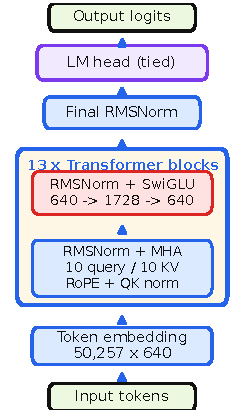
\includegraphics[width=\linewidth]{model1_architecture.pdf}
    \caption{Model~1: 13L, 96.64M.}
  \end{subfigure}\hfill
  \begin{subfigure}[t]{0.315\linewidth}
    \centering
    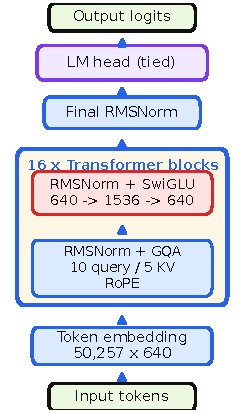
\includegraphics[width=\linewidth]{model2_architecture.pdf}
    \caption{Model~2: 16L, 99.03M.}
  \end{subfigure}\hfill
  \begin{subfigure}[t]{0.315\linewidth}
    \centering
    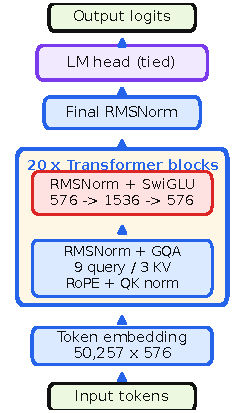
\includegraphics[width=\linewidth]{model3_architecture.pdf}
    \caption{Model~3: 20L, 99.78M.}
  \end{subfigure}
  \caption{Three sub-100M capacity allocations. GQA lets Models~2 and 3 trade
  independent key/value projections for greater depth.}
  \label{fig:architecture}
\end{figure}

\begin{table}[H]
  \caption{Exact capacity allocations for the starter and three candidate
  architectures. Parameters count tied embeddings once.}
  \label{tab:architecture-configs}
  \centering
  \small
  \setlength{\tabcolsep}{5pt}
  \begin{tabular}{@{}lrrrrcl@{}}
    \toprule
    Model & Layers & Width & Q/KV heads & MLP & QK norm & Parameters \\
    \midrule
    Starter & 8 & 512 & 8/8 & 2,048 & No & $<100$M \\
    Model~1 & 13 & 640 & 10/10 & 1,728 & Yes & 96.64M \\
    Model~2 & 16 & 640 & 10/5 & 1,536 & No & 99.03M \\
    Model~3 & 20 & 576 & 9/3 & 1,536 & Yes & 99.78M \\
    \bottomrule
  \end{tabular}
\end{table}

\paragraph{Block computation.}
For hidden state $h_\ell$, each pre-normalized residual block computes
\begin{align}
  u_\ell
    &= h_\ell +
       \operatorname{Attn}\!\left(\operatorname{RMSNorm}(h_\ell)\right),
       \label{eq:attn-block}\\
  h_{\ell+1}
    &= u_\ell + W_{\mathrm{down}}\!\left[
       \operatorname{SiLU}(W_{\mathrm{gate}}z_\ell)
       \odot W_{\mathrm{up}}z_\ell\right],
  \quad z_\ell=\operatorname{RMSNorm}(u_\ell).
  \label{eq:mlp-block}
\end{align}
RoPE is applied to queries and keys before causal scaled dot-product
attention. The output projection and SwiGLU down projection return to the
residual width, and the final language-model head shares weights with the
token embedding. The implementation uses no projection biases or dropout.

\paragraph{Capacity rationale.}
Let $d$ be the residual width and $r=h_{\mathrm{KV}}/h_{\mathrm{Q}}$. Ignoring
biases, the four attention projections require approximately
$d^2(2+2r)$ parameters per layer: $d^2$ each for queries and outputs and
$rd^2$ each for keys and values. Standard MHA has $r=1$ and costs $4d^2$;
the 1:2 and 1:3 GQA layouts cost approximately $3d^2$ and
$\frac{8}{3}d^2$. Models~2 and 3 reinvest those savings in three and seven
additional layers relative to Model~1. Because width, MLP size, GQA ratio,
and QK normalization also co-vary, the comparison supports complete
deep-and-thin designs rather than attributing the result to GQA alone.

\subsection{Optimization and Continuation}

\begin{wraptable}{r}{0.46\linewidth}
  \vspace{-0.8\baselineskip}
  \caption{Model~2 training configuration.}
  \label{tab:training-config}
  \centering
  \small
  \setlength{\tabcolsep}{4pt}
  \begin{tabular*}{\linewidth}{@{\extracolsep{\fill}}ll@{}}
    \toprule
    Hyperparameter & Value \\
    \midrule
    Context length & 1,024 \\
    Micro-batch & 16 sequences \\
    Global batch & 524,288 tokens \\
    Precision & bf16 autocast \\
    Gradient clipping & 1.0 \\
    Main-stage updates & 38,000 \\
    Warmup & 200 updates \\
    Peak Muon LR & $1.3{\times}10^{-2}$ \\
    Peak AdamW LR & $5.2{\times}10^{-4}$ \\
    Main LR floor & 10\% of peak \\
    \bottomrule
  \end{tabular*}
\end{wraptable}

Muon updates the two-dimensional hidden-layer matrices, while AdamW handles
embeddings and all other parameters. The main stage uses warmup followed by
cosine decay over 19.92B sampled tokens. An AdamW-only pilot improved
substantially more slowly.

Continuation restores weights, optimizer moments, data-loader cursors, and
random-number states. For Model~2, the Muon rate decreases from roughly
$3.0{\times}10^{-4}$ at step 38k to $3.0{\times}10^{-5}$ near step 69.7k;
AdamW remains at 4\% of that rate. Branches from 62k, 63.6k, and 69.6k shorten
the remaining cosine horizon and evaluate more frequently near convergence.
Architecture, batch, mixture, and objective remain fixed throughout; the
resulting gains therefore isolate continuation and checkpoint selection from
other modeling choices.

\begin{table}[H]
  \caption{Model~2 schedule and checkpoint-search stages. Learning rates are
  effective Muon rates observed in the logs; AdamW uses 4\% of each value.
  Monitoring gives the spacing between quick or official evaluations.}
  \label{tab:continuation-stages}
  \centering
  \small
  \setlength{\tabcolsep}{4.5pt}
  \begin{tabular}{@{}llllr@{}}
    \toprule
    Stage & Step range & Muon LR & Monitoring & Representative PPL \\
    \midrule
    Main training & 0--38.0k & $1.3{\times}10^{-2}\!\rightarrow1.3{\times}10^{-3}$ &
      2,000 & 21.163 \\
    Broad continuation & 38.0--62.0k &
      $3.00{\times}10^{-4}\!\rightarrow1.35{\times}10^{-4}$ &
      500--2,000 & 19.210 \\
    Short branch & 62.0--63.6k & $\approx7.7{\times}10^{-5}$ &
      100 & 19.096 \\
    Late branch & 63.6--69.6k &
      $5.10{\times}10^{-5}\!\rightarrow5.00{\times}10^{-5}$ &
      100 & 18.917 at 69.2k \\
    Final search & 69.6--71.8k & $\approx3.0{\times}10^{-5}$ &
      50 & \textbf{18.768 at 69.7k} \\
    \bottomrule
  \end{tabular}
\end{table}

\paragraph{Continuation as local search.}
The broad continuation determines whether the main checkpoint still has
optimization headroom. Once gains slow, each short branch starts from a
strong saved state, lowers the schedule scale, and increases measurement
frequency. This procedure is not weight averaging or fine-tuning on a new
dataset: every branch preserves the same model, source mixture, objective,
optimizer partition, and loader position. The only deliberate changes are
the remaining cosine horizon and the frequency of checkpoint evaluation.

\subsection{Design Rationale and Risk Controls}

Our hypothesis is that four changes compound: deeper GQA allocation, balanced
domains, the Muon--AdamW split, and low-rate continuation. The main risks are
interaction effects, validation overfitting, and unstable resume. Matched
pilots, full-state checkpoints, official validation, and conservative rates
control these risks. The starter model, FineWeb-Edu-only data, AdamW, and the
38k checkpoint remain usable fallbacks if a component fails.

\section{Experiments}
\label{sec:experiments}

\subsection{Baselines and Evaluation}

We use four complementary baseline families: \textbf{(i) Starter GPT}, the
8-layer nanoGPT-style model with learned positions, LayerNorm, GELU, and
AdamW; \textbf{(ii) single-source data}, FineWeb-Edu-only and
OpenWebText-only pilots under a shared short-run budget; \textbf{(iii) the
architecture family}, Models~1--3 under the same 50/20/15/15 mixture and
38k-update budget; and \textbf{(iv) an optimizer control}, AdamW versus
Muon + AdamW for Model~2 under a matched early-training budget.

The course evaluator computes token-weighted cross entropy over contiguous
1024-token chunks in \texttt{val.bin} and exponentiates the mean. Every full
evaluation covers 5,169,152 target tokens. Public-validation PPL is the
primary development metric; the hidden test is reserved for the course ranking
and is not used for schedule decisions. Internal mixed-shard validation losses
are used for trend monitoring but are not treated as directly comparable to
official PPL.

\subsection{Implementation Details}

Training uses PyTorch on a single NVIDIA L40S GPU with 48GB memory, bf16 mixed
precision, and scaled dot-product causal attention. Pure cross-entropy updates
take approximately eight seconds, so the selected 69.7k lineage alone
represents roughly 155 single-GPU hours before evaluation overhead. Additional
candidate and branch runs increase the full project cost. Because the corpus
is streamed and much larger than the sampled budget, an ``epoch'' is not a
literal pass over all documents. We therefore report updates and sampled
tokens; the best Model~2 checkpoint represents 36.54B sampled tokens.

Hyperparameter exploration includes depths $\{13,16,20\}$, FineWeb shares
$\{50,53,56\}\%$, standard MHA versus GQA, AdamW versus Muon + AdamW, and
progressively smaller continuation rates. Baseline runs are not all matched in
length; exact comparison budgets are listed in \cref{app:budgets}. The
training and exported configurations both use exactly 50,257 vocabulary
entries, and the tied output head therefore returns the evaluator-required
logit dimension directly.

\subsection{Reproducibility and State Integrity}
\label{sec:reproducibility}

\paragraph{Deterministic sampling.}
The source loader is seeded with 2025 and stores the shuffled 20-window cycle,
the position within that cycle, per-source shard indices and token cursors,
and the random-generator state. Within each source, cursors advance by one
non-overlapping context per process; reaching the end rotates to the next
memory-mapped shard. On resume, the code verifies that the distributed world
size matches the saved value before restoring the cursor state. These checks
prevent a nominal continuation from silently replaying windows or changing
the mixture.

\paragraph{Checkpoint and evaluation contracts.}
Training checkpoints contain model weights, both optimizer states, loader
state, CPU and CUDA random-number states, architecture configuration, and the
global step. Submission exports are separate minimal bundles containing
\texttt{model.py}, \texttt{config.json}, and raw model weights. At selected
steps, the training script exports this bundle and invokes the unmodified
course evaluator, which writes PPL, mean loss, token count, parameter count,
and evaluation time to JSON. Thus the plotted Model~2 points are linked to
evaluator-compatible artifacts rather than reconstructed from noisy
mini-batch losses.

\subsection{Main Results}
\label{sec:main-results}

\begin{table}[H]
  \caption{Public-validation checkpoints in the final model-selection
  progression. Lower PPL is better.}
  \label{tab:headline-results}
  \centering
  \small
  \setlength{\tabcolsep}{4.5pt}
  \begin{tabular}{@{}llllrr@{}}
    \toprule
    Model & Stage & Data mix & Split & Step & PPL \\
    \midrule
    Pilot baseline & short run & 50/20/15/15 & public val & 5k & 38.828 \\
    Model~1 & main & 56/18/13/13 & public val & 38k & 21.609 \\
    Model~1 & continuation & 56/18/13/13 & public val & 50.75k & 19.090 \\
    Model~2 & main & 50/20/15/15 & public val & 38k & 21.163 \\
    Model~2 & continuation & 50/20/15/15 & public val & 69.7k & \textbf{18.768} \\
    \bottomrule
  \end{tabular}
\end{table}

\Cref{tab:headline-results} summarizes the complete progression. The
short-run mixed-data baseline remains at 38.828 PPL, whereas the matched 38k
architecture runs reach the low 20s. Continuation improves Model~2 by another
2.395 PPL. We select the step-69.7k checkpoint with 18.768 PPL as the final
submission.

\begin{figure}[H]
  \centering
  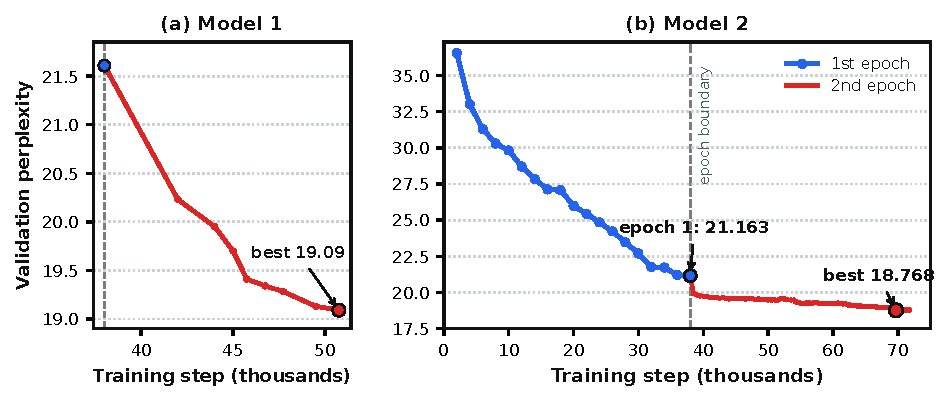
\includegraphics[width=0.90\linewidth]{training_curve.pdf}
  \caption{Low-rate continuation for Models~1 and 2. Red trajectories begin at
  the blue endpoints, preserving each checkpoint lineage. Model~1 values are
  team-reported; Model~2 values are log-verified.}
  \label{fig:training}
\end{figure}

\Cref{fig:training} shows that continuation transfers across architectures.
Model~1 improves from 21.609 to 19.09 by step 50.75k, an 11.7\% relative
reduction. Model~2 reaches 19.666 at 42k, 19.210 at 62k, 19.012 at 66k, and
18.768 at 69.7k. Later checkpoints fluctuate near 18.79--18.81; Model~1 is
similarly non-monotonic, worsening from 19.0900 to 19.1499 after another 500
updates. Evaluator-compatible checkpoint selection is therefore part of the
method rather than a reporting convenience.

\begin{table}[H]
  \caption{Marginal returns during Model~2 continuation. Added tokens count
  sampled training tokens within each interval; gains are not independent
  because later intervals inherit earlier checkpoints.}
  \label{tab:marginal-returns}
  \centering
  \small
  \setlength{\tabcolsep}{7pt}
  \begin{tabular}{@{}lrrrr@{}}
    \toprule
    Interval & Added tokens & Start PPL & End PPL & PPL reduction / B tokens \\
    \midrule
    38k $\rightarrow$ 42k & 2.10B & 21.163 & 19.666 & 0.714 \\
    42k $\rightarrow$ 62k & 10.49B & 19.666 & 19.210 & 0.043 \\
    62k $\rightarrow$ 69.7k & 4.04B & 19.210 & 18.768 & 0.110 \\
    \bottomrule
  \end{tabular}
\end{table}

\paragraph{Training dynamics.}
The first 4k continuation updates deliver the largest return, reducing PPL by
1.497 with 2.10B additional tokens. The next 20k updates improve more slowly,
whereas the short late branches recover a larger gain per token by lowering
the rate and searching densely near a strong state. Branch selection itself
consumes evaluation effort, so this is not proof of compute optimality; it
does show that one checkpoint interval is poorly matched to both phases.

\paragraph{Checkpoint sensitivity.}
The best point is narrow rather than a stable terminal plateau. Official
evaluation gives 18.768 at 69.7k, 18.776 at 70.0k, and 18.799 at 71.8k.
Selecting the last state would discard a measurable verified gain without
changing training compute, architecture, or data.

\subsection{Controlled Comparisons}
\label{sec:ablations}

\begin{table}[H]
  \caption{Observed effect sizes within each controlled comparison or
  checkpoint lineage. Relative reduction uses the worse setting as the
  denominator; rows have different training budgets and are not additive.}
  \label{tab:effect-sizes}
  \centering
  \small
  \setlength{\tabcolsep}{6pt}
  \begin{tabular}{@{}llrr@{}}
    \toprule
    Intervention & Comparison & Absolute PPL reduction & Relative reduction \\
    \midrule
    Data source & OpenWebText $\rightarrow$ mixture & 26.382 & 40.5\% \\
    Source weights & 56/18/13/13 $\rightarrow$ 50/20/15/15 & 0.284 & 1.3\% \\
    Capacity allocation & Model~1 $\rightarrow$ Model~3 & 0.407 & 1.9\% \\
    Optimizer & AdamW $\rightarrow$ Muon + AdamW & 3.433 & 8.6\% \\
    Model~1 continuation & 38k $\rightarrow$ 50.75k & 2.519 & 11.7\% \\
    Model~2 continuation & 38k $\rightarrow$ 69.7k & 2.395 & 11.3\% \\
    \bottomrule
  \end{tabular}
\end{table}

The effect-size view clarifies the project priorities. Choosing an unsuitable
source overwhelms the architecture-scale differences, while the optimizer
split and continuation each produce substantially larger relative gains than
the matched 38k architecture change. Architecture still determines the state
from which optimization continues, and a 0.4-PPL difference remains meaningful
near the final operating point.

\begin{table}[H]
  \caption{Detailed validation ablations. Rows are matched within each factor;
  exact budgets appear in \cref{app:budgets}. Lower PPL is better.}
  \label{tab:ablations}
  \centering
  \normalsize
  \renewcommand{\arraystretch}{1.06}
  \setlength{\tabcolsep}{12pt}
  \begin{tabular}{@{}llr@{}}
    \toprule
    Factor & Setting & PPL \\
    \midrule
    Data source & FineWeb-Edu only & 39.670 \\
                & OpenWebText only & 65.210 \\
                & Four-source mixture & \textbf{38.828} \\
    \midrule
    FineWeb share & 50/20/15/15 & \textbf{21.325} \\
                  & 53/19/14/14 & 21.460 \\
                  & 56/18/13/13 & 21.609 \\
    \midrule
    Architecture & Model~1: 13L, MHA & 21.325 \\
                 & Model~2: 16L, GQA 1:2 & 21.163 \\
                 & Model~3: 20L, GQA 1:3 & \textbf{20.918} \\
    \midrule
    Optimizer & AdamW & 39.973 \\
              & Muon + AdamW & \textbf{36.540} \\
    \midrule
    LR branch & $1.35{\times}10^{-4}$ & 19.218 \\
              & $1.03{\times}10^{-4}$ & 19.152 \\
              & $7.74{\times}10^{-5}$ & \textbf{19.103} \\
    \bottomrule
  \end{tabular}
\end{table}

\Cref{tab:ablations} shows that the four-source mixture improves over
FineWeb-Edu-only by 0.842 PPL and over OpenWebText-only by 26.382. Raising the
FineWeb-Edu share from 50\% to 53\% or 56\% hurts Model~1 by 0.135 and 0.284
PPL. Thus, the strongest source need not deserve a larger share.

At 38k, Model~2 beats Model~1 by 0.162 PPL, and Model~3 gains another 0.245.
Because width and QK normalization also vary, this supports the complete
deeper designs rather than GQA alone. In the matched optimizer pilot, Muon +
AdamW reduces PPL from 39.973 to 36.540, an 8.6\% relative gain.

\paragraph{Learning-rate refinement.}
We branch Model~2 three ways from the same 62k checkpoint and train each for
800 updates. Lowering the effective starting Muon LR from
$1.35{\times}10^{-4}$ to $1.03{\times}10^{-4}$ and
$7.74{\times}10^{-5}$ improves PPL at 62.8k from 19.218 to 19.152 and 19.103,
respectively. We retain the lowest-rate branch, which reaches 19.096 at 63.6k.
Restarting at $5.10{\times}10^{-5}$ then reaches 18.781 at 69.6k, and a final
$3.01{\times}10^{-5}$ branch reaches 18.768 after 100 updates. These later
stages inherit selected checkpoints and use unequal budgets, so they document
the successful search trajectory rather than independent matched ablations.

\subsection{Negative Findings}

Several negative results changed our procedure. OpenWebText-only training was
not competitive; increasing the strongest source from 50\% to 56\% degraded
Model~1; and the final continuation checkpoint was not the best checkpoint.
Model~3 was strongest at 38k, beating Model~2 by 0.245 PPL, so we do not claim
that Model~2 is the globally best architecture. We continued Model~2 because
its complete model, optimizer, loader, and random states were available for a
controlled resume. A fair final architecture ranking would require the same
continuation and checkpoint-selection budget for all three models.

\section{Discussion}
\label{sec:discussion}

\paragraph{Achievements and lessons.}
We train a competitive sub-100M model, reducing public-validation PPL from
38.828 in a short pilot to 18.768 at the selected submission checkpoint. Our
architecture study favors deeper GQA designs under a fixed parameter cap,
while continuation yields the largest within-model improvement. More broadly,
the model, data loader, optimizer, and checkpoint policy form one system;
architecture-only optimization leaves substantial performance unused.

\paragraph{Selection validity.}
Repeated use of one public validation set creates selection bias, especially
when checkpoints are evaluated every 50--100 updates. We mitigate this concern
by keeping \texttt{val.bin} out of training and changing only schedule
parameters after the architecture and data mixture are fixed. This does not
quantify the full uncertainty introduced by branch selection. A stronger
protocol would reserve a second local validation mixture for schedule
decisions and use the public evaluator only for sparse confirmation.

\Needspace{8\baselineskip}
\paragraph{Compute allocation.}
The selected lineage processes 19.92B tokens before continuation and another
16.62B by the best checkpoint. The marginal-return analysis shows that these
tokens are not equally valuable: the first 2.10B continuation tokens produce
most of the immediate gain, whereas later progress depends on smaller rates
and denser measurement. Near convergence, a full official evaluation can take
several minutes, so evaluating every saved checkpoint becomes a meaningful
fraction of wall-clock cost. Coarse evaluation is appropriate early; dense
evaluation is justified only once successive training updates move PPL by
hundredths.

\paragraph{Systems lesson.}
Exact continuation required more than loading model weights. Restoring both
optimizers, loader cursors, source-cycle order, and random states preserved the
meaning of a global training step and avoided data replay. Separating rich
training checkpoints from minimal submission bundles also reduced the risk of
exporting optimizer state or an incompatible configuration. These engineering
choices do not directly change the loss function, but they make the late-stage
gains auditable and reproducible.

\paragraph{Bottlenecks and limitations.}
Full-scale controlled experiments are expensive, so not every candidate
receives the same continuation budget. The architecture comparison changes
multiple dimensions at once and should not be interpreted as a factorial
ablation. Validation-driven branching can also over-specialize to
\texttt{val.bin}; without an independent local holdout, we cannot quantify
this effect. Experiment metadata is distributed across logs, model cards, and
presentation records, making provenance harder to audit than a unified
experiment tracker.

\paragraph{Future work.}
Future experiments should allocate equal sampled-token budgets and
checkpoint-selection effort to all three architectures. A second held-out
mixture would reduce schedule overfitting, while automated evaluation and
best-checkpoint retention would remove manual branching. More systematic
mixture optimization could replace the coarse 50/53/56\% sweep, and matched
throughput measurements could separate parameter efficiency from realized
training speed, memory use, and inference latency under deployment constraints.

\section{Team Contributions and LLM Usage}

\begin{itemize}
  \item \textbf{Yirui Miao:} experiment planning; analysis of data and
  architecture choices; ablation interpretation; report and presentation
  synthesis.
  \item \textbf{Fengfei Yu:} Model~2 training and continuation; evaluation and
  export infrastructure; log consolidation; result verification.
  \item \textbf{Tianyue Zhang:} data-mixture experiments; result synthesis;
  report analysis and writing.
  \item \textbf{Zavier Zhao:} Model~1 development; baseline and mixture
  experiments; presentation and report writing.
\end{itemize}

\paragraph{LLM usage.}
Large language models were used as writing and code-review assistants for
summarizing local experiment notes, drafting report prose, and checking
organization. The team remains responsible for all reported experimental
claims, and numerical claims in this report were taken from the repository
logs, model cards, code, or the team's presentation notes.

\clearpage
\bibliography{references}
\bibliographystyle{plainnat}

\clearpage
\appendix

\section{Evaluation Budgets}
\label{app:budgets}

\begin{table}[h]
  \caption{Matched evaluation points for the comparisons in
  \cref{tab:ablations}.}
  \label{tab:ablation-budgets}
  \centering
  \small
  \begin{tabular}{@{}lll@{}}
    \toprule
    Factor & Compared settings & Evaluation update \\
    \midrule
    Data source & FineWeb-Edu, OpenWebText, mixture & 5,000 \\
    FineWeb share & 50\%, 53\%, 56\% in Model~1 & 38,000 \\
    Architecture & Models~1--3, 50/20/15/15 mix & 38,000 \\
    Optimizer & AdamW, Muon + AdamW in Model~2 & 2,000 \\
    LR branch & Three Model~2 rates from the same 62k state & 62,800 \\
    \bottomrule
  \end{tabular}
\end{table}

\section{Architecture and Reproducibility Details}

\begin{table}[h]
  \caption{Model~2 code, checkpoints, and final evaluation records.}
  \label{tab:repro-paths}
  \centering
  \small
  \begin{tabular}{@{}lp{0.68\textwidth}@{}}
    \toprule
    Artifact & Repository location or value \\
    \midrule
    Main training & \path{build-nanogpt/train_gpt2_v13.py} \\
    Continuation & \path{build-nanogpt/train_gpt2_v16.py} \\
    Main checkpoint & \path{build-nanogpt/log/v13/train_ckpt_38000.pt} \\
    Best exported checkpoint &
    \path{build-nanogpt/log/v16/.../submission_..._69700} \\
    Best public validation & Step 69,700; PPL 18.7681466; loss 2.932161 nats \\
    Code repository & \url{https://github.com/ty1erz/cse251b-nanogpt} \\
    \bottomrule
  \end{tabular}
\end{table}

\end{document}
